% LaTeX-ready figure environment for the multi-seed fall-recall-vs-epsilon plot.
% Image: figures/multiseed_robustness/multiseed_fall_recall_vs_epsilon.png
% Source data commit: 3200a89 (branch feature/converged-clean-baseline)
% Requires \usepackage{graphicx}.

\begin{figure}[t]
  \centering
  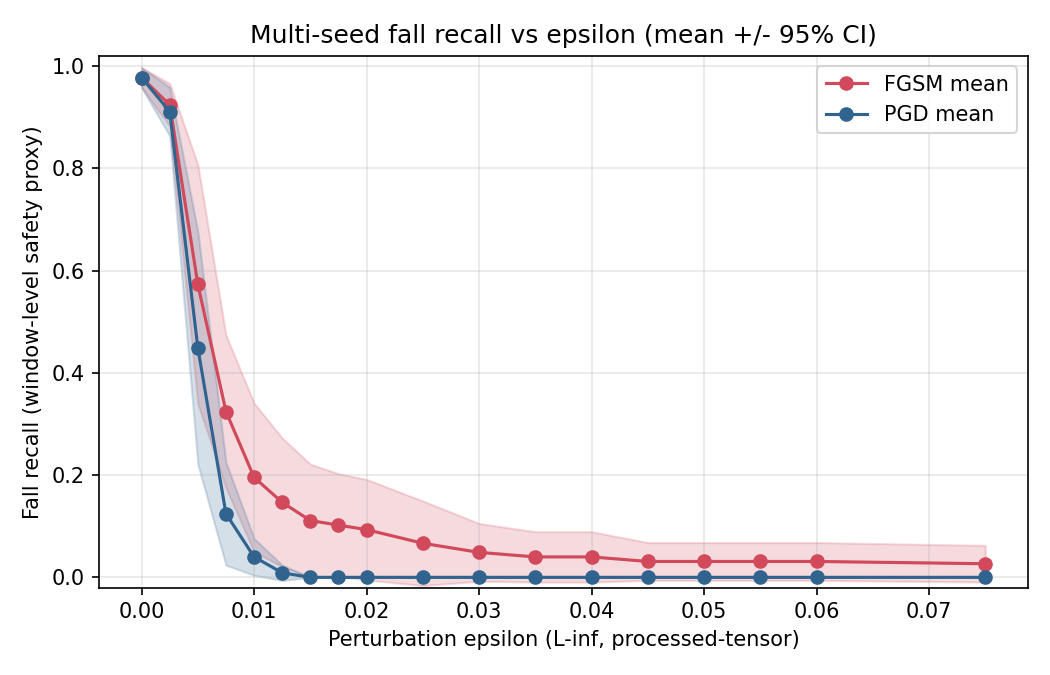
\includegraphics[width=0.8\linewidth]{figures/multiseed_robustness/multiseed_fall_recall_vs_epsilon.png}
  \caption[Multi-seed fall recall vs.\ perturbation budget]{%
    Window-level fall recall versus $L_\infty$ perturbation budget $\varepsilon$
    for undefended FGSM and PGD attacks on the UT-HAR/SenseFi LeNet classifier,
    aggregated over five independent training seeds (42--46). Solid lines are the
    per-$\varepsilon$ mean across seeds; shaded bands are 95\% confidence
    intervals (Student-$t$, $df=4$). Perturbations are digital-domain,
    processed-tensor perturbations on the held-out test split ($n=500$ windows,
    $45$ fall windows); they are not physical-layer or over-the-air attacks.
    Clean fall recall ($\varepsilon=0$) is $0.978\pm0.016$; PGD drives recall to
    $0.000$ in every seed by $\varepsilon\approx0.0125$, and FGSM to near zero by
    $\varepsilon\approx0.037$.}
  \label{fig:multiseed-fall-recall-vs-epsilon}
\end{figure}
